\section{Logic-of-Thought Routing}
\label{sec:lotr}

\subsection{Problem Formulation}
\label{sec:formulation}

Let $f_\theta$ be a frozen Transformer with $L$ layers, where layer $\ell$ contains $H_\ell$ attention heads, and let $\mathcal{H}=\{(\ell,h)\mid \ell\in\{1,\dots,L\},\, h\in\{1,\dots,H_\ell\}\}$ denote the heads. For an input problem $x$, let $p$ be the prompt constructed under a fixed external \emph{reasoning strategy} $\pi$, and let $y_{1:T}=(y_1,\ldots,y_T)$ denote the resulting reasoning trajectory, where each $y_t$ is a sentence-level reasoning step. 
%We set $y_{<1}=\varnothing$, so the first pathway is initialized from the prompt-induced logic state before any reasoning step is generated. 
Under such a strategy, each reasoning step is produced through head-level information transfer across layers, so the internal execution of reasoning can be viewed through the pattern of head participation.

To make this view operational, we introduce a step-level \emph{internal computation pathway} 
$\mathcal{P}_t=\{\gamma_t^{(\ell,h)}\}_{(\ell,h)\in\mathcal{H}}$, 
where $\gamma_t^{(\ell,h)}\in[0,1]$ denotes the participation strength assigned to head $(\ell,h)$ when producing step $t$.
Rather than assuming a discrete or uniquely identifiable circuit, $\mathcal{P}_t$ serves as a soft pathway descriptor over attention heads.
The induced step-level generation can then be written as 
$p(y_t\mid p,y_{<t};\pi,\mathcal{P}_t)$.
The central problem of LoTR is to characterize the \emph{reasoning logic} induced by the fixed external strategy at the current step (Sec.~\ref{sec:offline}), and to instantiate a soft internal pathway $\mathcal{P}_t$ that is better matched to that logic (Sec.~\ref{sec:online}), as shown in Figure~\ref{fig:intro_main} and Algorithm~\ref{alg:lotr_pipeline}.
% Section~\ref{sec:offline} builds a compact basis of recurring logic states together with their associated pathway templates, and Section~\ref{sec:online} shows how these templates are invoked during reasoning.
\vspace{-0.5mm}

\subsection{Offline Logic Modeling}
\label{sec:offline}
\vspace{-0.5mm}

The offline stage builds a compact basis of recurring logic states and couples them to stable head-level pathway patterns with details in Appendix~\ref{app:alg_offline}. This shifts the structural computation away from inference time, so the online controller only needs lightweight readout and template composition.

\vspace{-0.5mm}
\textbf{Logic-state basis.}
We first collect reasoning trajectories from diverse reasoning paradigms and pool their step-level representations into a shared bank. For each reasoning step $t$, we extract a compact reference readout $r_t=\phi(p,y_{\le t};f_\theta)\in\mathbb{R}^d$, instantiated as the mean-pooled hidden representation over the current sentence span from the final block. 
% Here, $d$ is the model hidden dimension of the readout space. 
Pooling across paradigms is essential: LoTR treats logic as a shared internal basis rather than as a byproduct of any single external strategy.

We then cluster the pooled readouts $\mathcal{R}=\{r_t\}$ into $K$ groups and use the resulting centroids $\{c_k\}_{k=1}^K$ as anchors of the recurring logic states, with $\mathcal{C}_k$ denoting the set of steps assigned to centroid $c_k$.The number of states is selected by a clustering-quality criterion such as silhouette score~\citep{rousseeuw1987silhouettes}, so that the basis remains compact while preserving meaningful separation. Because a reasoning step may reflect mixed logic rather than a single pure mode, we use soft state targets:
\begin{equation}
\alpha_t^\star(k)=\exp\!\left(-\frac{\|r_t-c_k\|_2^2}{\tau d_k^2}\right), \qquad k=1,\dots,K,
\label{eq:lotr_soft_target}
\end{equation}
where $d_k$ is an effective radius of cluster $k$ and $\tau$ is a temperature with stress tests in Sec.~\ref{sec:param_stress}. This target measures how strongly step $t$ aligns with state $k$ without forcing competition across states.
\vspace{-0.5mm}

\textbf{Layer-wise logic probes.}
To make the state basis usable online, LoTR trains a lightweight linear probe at each routed layer~\citep{alain2016understanding}. For layer $\ell\in\mathcal{L}_{\mathrm{route}}$, let $r_t^{(\ell)}\in\mathbb{R}^d$ be the sentence-level readout extracted from layer $\ell$, using the same sentence span and the same pooling rule as above. The probe predicts a non-exclusive state mixture
\begin{equation}
q_t^{(\ell)}=\sigma\!\left(A^{(\ell)}r_t^{(\ell)}+b^{(\ell)}\right)\in(0,1)^K,
\label{eq:lotr_probe}
\end{equation}
where $\sigma(\cdot)$ is the element-wise sigmoid. We deliberately avoid simplex-constrained normalization, since multiple logic states may co-activate within the same reasoning step. The probes are trained by binary cross-entropy against the soft state targets:
\begin{equation}
\mathcal{L}_{\mathrm{probe}}
=
-\sum_{\ell\in\mathcal{L}_{\mathrm{route}}}
\mathbb{E}_{t}
\sum_{k=1}^{K}
\Big[
\alpha_t^\star(k)\log q_t^{(\ell)}(k)
+
\big(1-\alpha_t^\star(k)\big)\log\!\big(1-q_t^{(\ell)}(k)\big)
\Big].
\label{eq:lotr_probe_loss}
\end{equation}

\vspace{-0.5mm}
\textbf{Logic--pathway coupling.}
With the state basis fixed, we next couple each state to a stable head-level pathway template. Let $v_{\ell,h}(t)\in\mathbb{R}^d$ denote the mean-pooled output of head $(\ell,h)$ over the sentence span at step $t$, measured in the same hidden space as the state readouts. $u_k=c_k/\|c_k\|_2$ is the normalized direction of centroid $c_k$, we then define the state-conditioned importance of head $(\ell,h)$ as
\begin{equation}
I_{\ell,h,k}
=
\mathbb{E}_{t:\, r_t\in\mathcal{C}_k}
\left[
\frac{\big(u_k^\top v_{\ell,h}(t)\big)^2}
{\|v_{\ell,h}(t)\|_2^2+\epsilon}
\right].
\label{eq:lotr_importance}
\end{equation}
This score is large when the head consistently contributes in a direction aligned with state $k$, and small when its contribution is weak or state-insensitive. We normalize $\{I_{\ell,h,k}\}_{h=1}^{H_\ell}$ and then obtain a state-specific pathway template $M_k=\{m_k^{(\ell,h)}\}_{(\ell,h)\in\mathcal{H}}$. Heads whose importance varies little across states naturally receive near-identity weights across templates, so the effective differences remain concentrated on the smaller subset of logic-sensitive heads.

Therefore, this offline stage yields a shared logic space in which different reasoning paradigms can be compared directly. Although their external strategies differ, they need not occupy that space in the same way: some repeatedly concentrate on a few states, whereas others traverse a broader or more mixed subset as shown in Figure~\ref{fig:lotr_logic_states}. This leads to the first structural observation behind LoTR: external reasoning paradigms differ not only in their trajectory-level procedures, but also in the distributions they induce over latent internal states.
We call these states \emph{logic states} because they appear as recurring, probe-identifiable execution regimes along reasoning trajectories, and later validate their functional relevance through state-conditioned routing and ablation analyses.

\begin{figure}[!t]
    \centering
    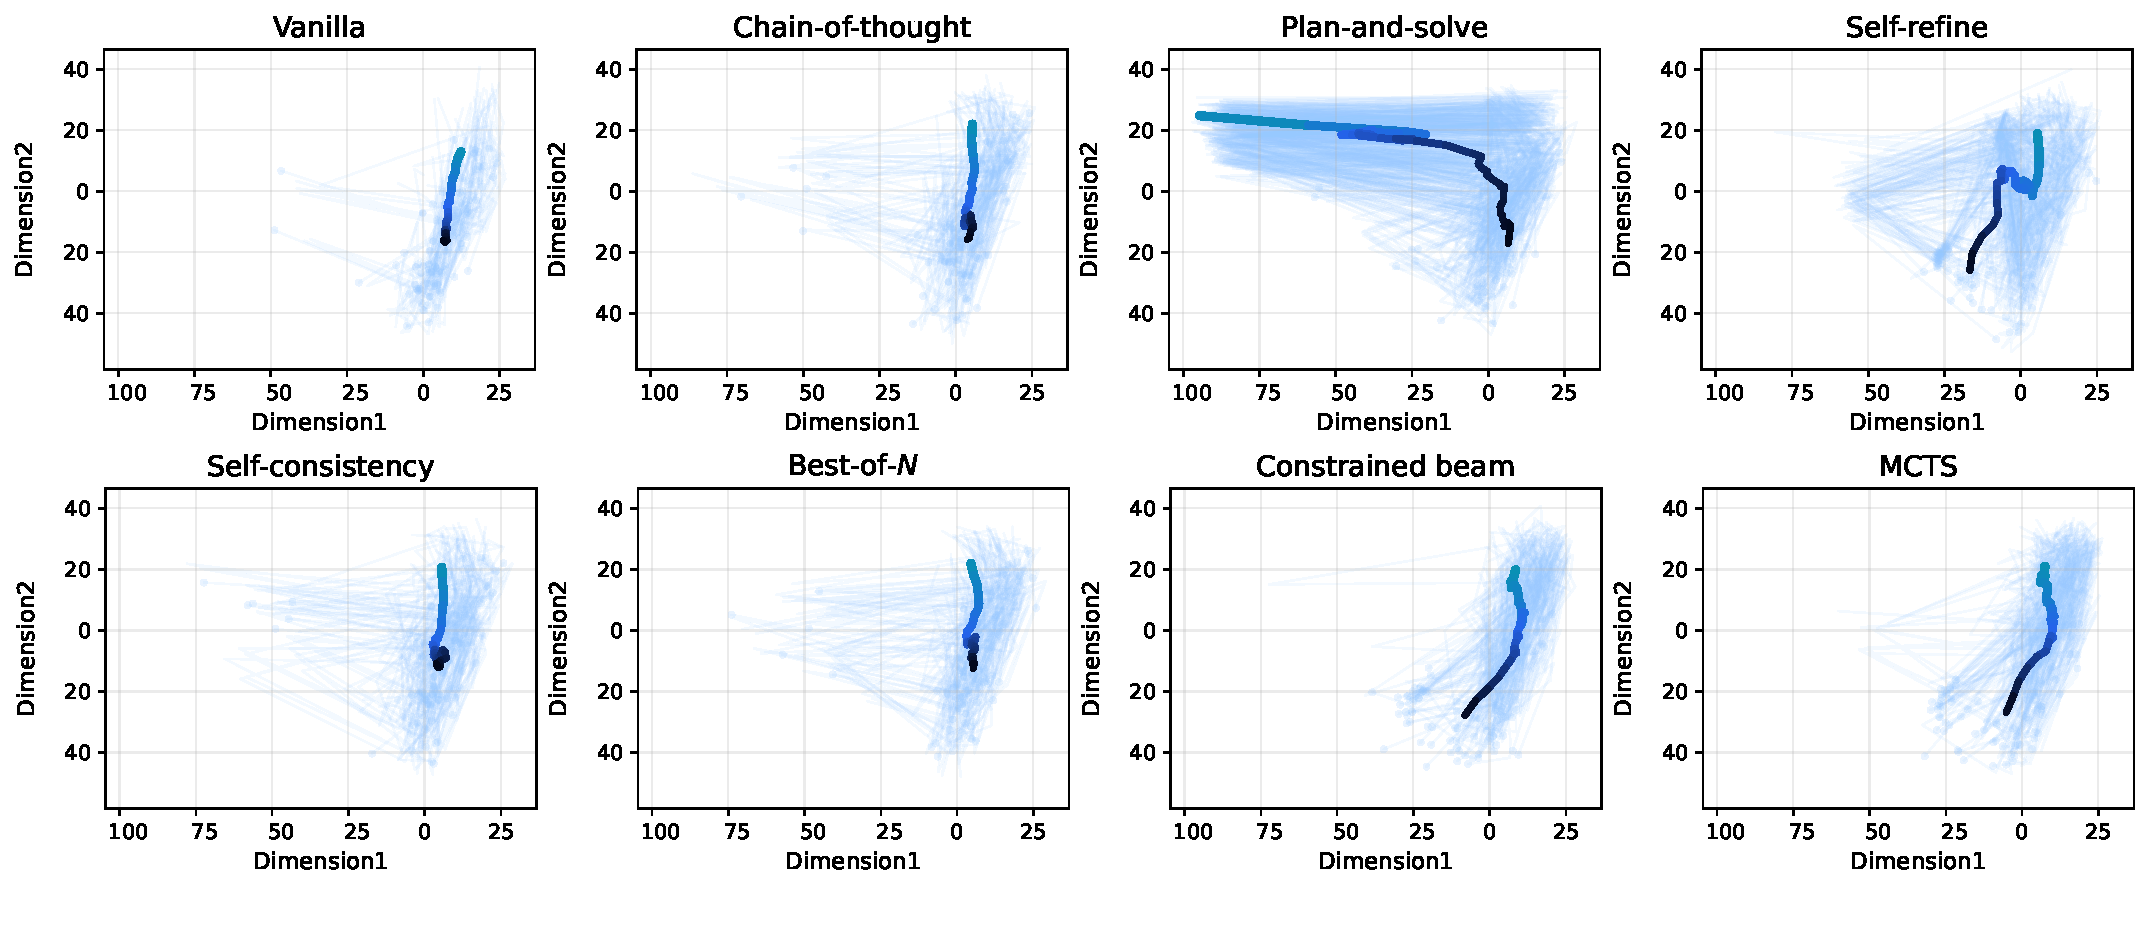
\includegraphics[width=1.00\textwidth]{figs/logicstate_paradigm_trajectories_pca2_grid.pdf}
    \vspace{-3mm}
    \caption{
    \textbf{Logic states across reasoning paradigms}. Different external strategies occupy different regions and transition patterns, suggesting distinct distributions over the same latent logic-state space.
    }
    \vspace{-3mm}
    \label{fig:lotr_logic_states}
\end{figure}

\vspace{-0.5mm}
\subsection{Online Probe-Based Plug-in Reasoning}
\label{sec:online}
\vspace{-0.5mm}

\textbf{Pathway instantiation.}
As reasoning unfolds, LoTR dynamically reads the layer-wise sentence representations $\{r_t^{(\ell)}\}_{\ell\in\mathcal{L}_{\mathrm{route}}}$ and evaluates the trained probes in Eq.~\eqref{eq:lotr_probe}. The resulting activations $\{q_t^{(\ell)}\}$ provide a compact state-level description of the logic currently expressed by the ongoing step.

LoTR then composes the pathway for the subsequent step by mixing the cached state templates according to these activations. For each routed layer $\ell$ and head $(\ell,h)\in\mathcal{H}$, we compute
\begin{equation}
\gamma_{t+1}^{(\ell,h)}
=
\mathrm{clip}\!\left(
\sum_{k=1}^{K} q_t^{(\ell)}(k)\, m_k^{(\ell,h)},
\,0,\,1
\right),
\qquad (\ell,h)\in\mathcal{H},
\label{eq:lotr_routing}
\end{equation}
which instantiates the pathway $\mathcal{P}_{t+1}=\{\gamma_{t+1}^{(\ell,h)}\}_{(\ell,h)\in\mathcal{H}}$ for generating step $y_{t+1}$, with the coefficients directly applied to the corresponding head outputs.

\textbf{Plug-in reasoning.}
The resulting controller is lightweight: online inference requires only one probe evaluation per layer at each sentence boundary, followed by a weighted combination over cached templates, with details in Appendix~\ref{app:alg_online}. This simple state-to-pathway map is already sufficient to make internal execution adaptive to the dynamic reasoning logic induced by a fixed external strategy.

Figure~\ref{fig:lotr_pathway_patterns} illustrates the second structural observation behind LoTR: the discovered logic states behave as recurring internal regimes, rather than merely isolated hidden-state clusters, and are empirically coupled to distinct head-level routing patterns that can be reused during reasoning.
In this sense, LoTR does not alter the external reasoning paradigm itself; instead, it improves its execution by aligning each reasoning step with an internal pathway suited to the logic state it currently induces.

\begin{figure}[!t]
    \centering
    \vspace{-2mm}
    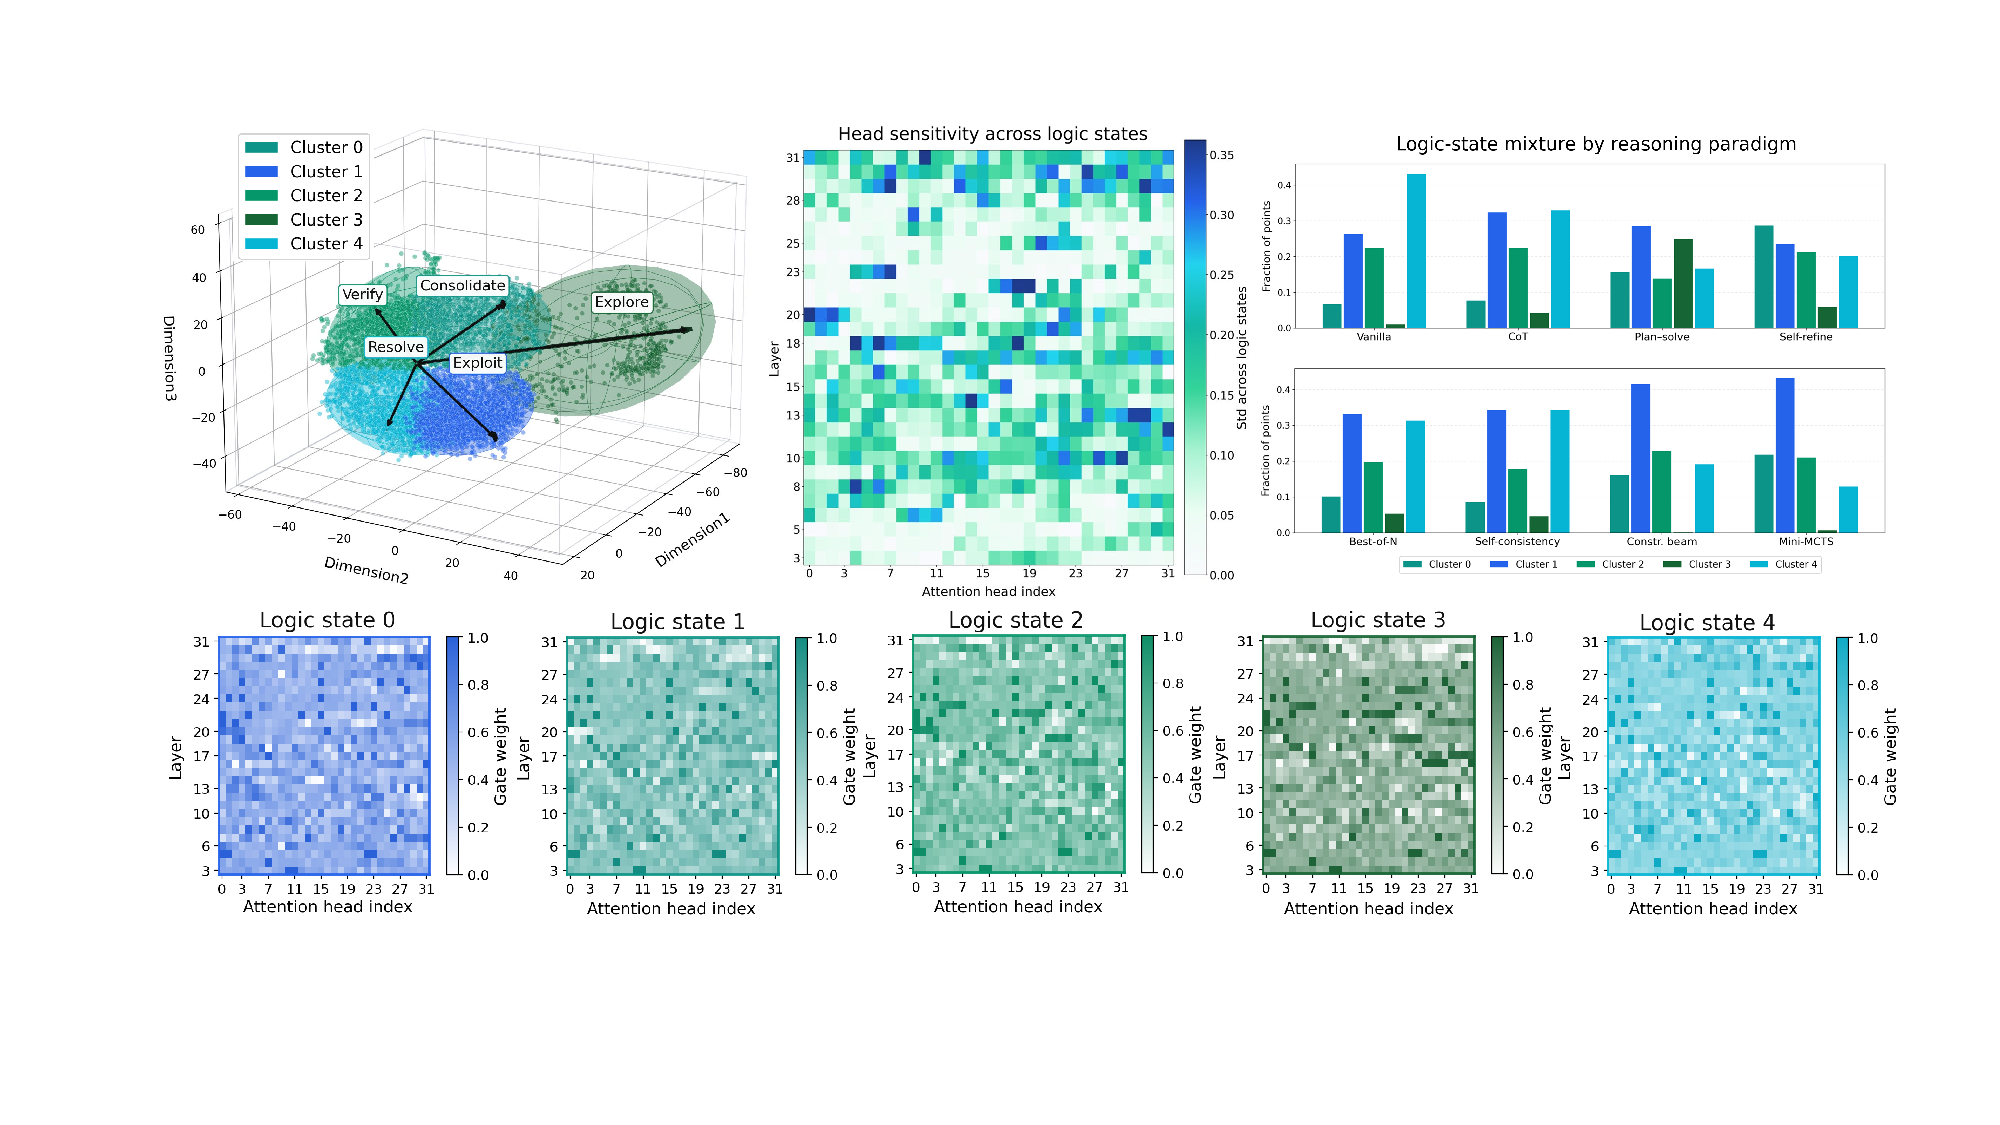
\includegraphics[width=0.9\textwidth]{figs/lotr_pathway_patterns.pdf}
    \vspace{-1mm}
    \caption{
    \textbf{Stable pathway patterns under different logic states.}
    Distinct recurring logic states are coupled to distinct head-level routing templates, enabling reusable pathway control.
    }
    \label{fig:lotr_pathway_patterns}
    \vspace{-3mm}
\end{figure}